\chapter{Concept and Design}
\label{cha:conceptanddesign}
 
The standards presented in \autoref{cha:relatedwork} show the potential improvements that can be achieved in key components of ActiviyPub-based social networks. In this chapter, the design that combines these standards with an actual ActivityPub implementation will be presented. As mentioned in \autoref{cha:relatedwork}, the proposal presented in this chapter and the modus operandi of the ActivityPub server is going to be scoped to the actual implementation in Mastodon.

The outline for this chapter is the following. First, individual concepts of the ActivityPub implementation are explained. Then, a use case example is going to be illustrated and step-by-step explained to be able to compare it with \autoref{section:did_flow}, which finally presents the same use case but this time with the proposed concept and design that includes DID integration and DIDComm enablement.
 
\section{Definitions}
Mastodon has implemented its own ActivityPub server, and with it also its own terms to express different social network vocabulary. To prevent confusion or ambiguities, the used terms in this chapter are explained here. 
 
\begin{itemize}
  \item \textbf{Username}: The username in Mastodon consists of a unique local username and the domain of the instance. Ex. alice@example.com
  \item \textbf{Actor object}: In this section, the term \emph{Actor object} refers solely to the ActivityPub's actor object. 
  \item \textbf{Status}: In the backend of Mastodon, the class used for a Toot is a Status. An account in Mastodon has a 1:n relationship with statuses.
\end{itemize}

\section{Use Case}\label{section:use_case}
To explain the current ActivityPub flow in Mastodon, the following use case will be used:

\emph{Alice has an account in the Mastodon instance alice\_server.com. Alice follows Bob, who has an account in the Mastodon instance bob\_server.com. Alice sends a direct message to Bob with the text: "Hello Bob!" }

\pagebreak

\section{Mastodon's Implementation}
In this section, each step required for the use case to be successful will be explained. At the end of this section, there is a sequence diagram, figure \ref{fig:normal_flow}, that provides an overview of the whole process, with a reference to every step. 

\subsection{Activity Creation}
The first thing that happens when Alice presses the send button is the creation of an ActivityStreams object. In this case, the object is of type \emph{Note} and will be created by Alice's server, as shown in \ref{fig:create_note}. Then, following the ActivityPub pattern of "some activity by some actor being taken on some object"\cite{lemmer-webber_tallon_guy_prodromou_2018}, the server wraps it in a \emph{Create} activity. The activity includes Alice in the \emph{attributeTo} field \ref{fig:create_activity}. Now that the actor, the activity, and the object are well defined and wrapped, it is time to shift our focus to the recipients of this note object. 
Alice's server will now look at the fields to, bto, cc, bcc, and audience to retrieve the recipients. Depending on where the recipient's account lives, Alices' server may take one of two options. If the recipient's account is on the same server, a simple query in the server would find the right account and save the status to the account's collection. Nonetheless, the use case explicitly dictates that Bob's account resides in a different Mastodon instance, namely \emph{bob\_server.com}. Therefore, a resolving process must be started.

% Note Object with content: 'Hello Bob'
\lstset{style=JSONStyle}
\begin{lstlisting}[language=PHP, caption=ActivityStreams note object, label=fig:create_note]
  {
    "@context": "https://www.w3.org/ns/activitystreams",
    "type": "Note",
    "to": "http://bob_server.com/users/bob",
    "attributedTo": "http://alice_server.com/users/alice",
    "content": "Hello Bob!"
  }
\end{lstlisting}

\lstset{style=JSONStyle}
\begin{lstlisting}[language=PHP, caption=ActivityStreams create activity, label=fig:create_activity]
  {
    "@context": "https://www.w3.org/ns/activitystreams",
    "type": "Create",
    "id": "https://alice_server/users/alice/statuses/634367/activity",
    "to": "http://bob_server.com/users/bob",
    "actor": "http://alice_server.com/users/alice",
    "object": {
      "type": "Note",
      "to": "http://bob_server.com/users/bob",
      "attributedTo": "http://alice_server.com/users/alice",
      "content": "Hello Bob!"
    }
  }
\end{lstlisting}

\subsection{DNS-based Resolving Process}
 Resolving is the fundamental part of the federated side of Mastodon. Without it, users within different instances would not be able to interact, as the instance itself does not know where to find the actor object with all required endpoints to send or receive activities from and to external accounts. For this reason, the current way to look up other accounts is through the DNS. In the same way Email works, the domain part of the username in Mastodon points to the domain of the instance where the account lives. The purpose of resolving is to find Bob's inbox URL, which can be found in Bob's actor object. As explained in \autoref{cha:relatedwork}, Mastodon includes a series of well-known endpoints that are used to retrieve information about resources managed by the host. As Bob's account lives inside \emph{bob\_server.com}, Mastodon triggers a Webfinger request to Bob's server. This request returns a JRD Document, as shown in listing \ref{fig:webfinger_request} and \ref{fig:webfinger_response}. Based on this document, Alice's server retrieves the link with the \emph{rel: 'self'} which includes the type and the URL where Bob's actor object can be retrieved. A subsequent HTTP GET request to this URL with the specific \emph{application/activity+json} header will return Bob's actor object \ref{fig:bob_object}. If the Webfinger request \ref{fig:hostmeta_request} returns a 404 code, it will then try, as a fallback, using the Host-Meta endpoint. The response contains a link template \ref{fig:hostmeta_response}, that Alice's server can use to try the Webfinger request again.  

\begin{lstlisting}[language=PHP, caption=Webfinger request to \emph{bob\_server.com}, label=fig:webfinger_request]
  GET /.well-known/webfinger?resource=acct:bob@bob_server.com HTTP/1.1
  Host: bob_server.com
  Accept: application/ld+json
\end{lstlisting}

\lstset{style=JSONStyle}
\begin{lstlisting}[language=PHP, caption=Webfinger response from \emph{bob\_server.com}, label=fig:webfinger_response, float=h]
  {
    "subject": "acct:bob@bob_server.com",
    "aliases": [
      "https://bob_server.com/@bob",
      "https://bob_server.com/users/bob"
    ],
    "links": [{
        "rel": "http://webfinger.net/rel/profile-page",
        "type": "text/html",
        "href": "https://bob_server.com/@bob"
      },
      {
        "rel": "self",
        "type": "application/activity+json",
        "href": "https://bob_server.com/users/bob"
      },
    ]
  }
\end{lstlisting}

\pagebreak

\begin{lstlisting}[language=PHP, caption=Host-Meta request to \emph{bob\_server.com}, label=fig:hostmeta_request, float=h]
  GET /.well-known/host-meta HTTP/1.1
  Host: bob_server.com
  Accept: application/xrd+xml
\end{lstlisting}

\lstset{style=JSONStyle}
\begin{lstlisting}[language=PHP,caption=Host-Meta response from \emph{bob\_server.com}, label=fig:hostmeta_response, float=h]
  <?xml version="1.0" encoding="UTF-8"?>
  <XRD xmlns="http://docs.oasis-open.org/ns/xri/xrd-1.0">
      <Link rel="lrdd" template="https://bob_server.com/.well-known/webfinger?resource={uri}"/>
  </XRD>
\end{lstlisting} 

%  Actor Object ActivityPub
\lstset{style=JSONStyle}
\begin{lstlisting}[language=PHP, caption=Bob's actor object, label=fig:bob_object, float=h!]
  {
    "@context": "https://www.w3.org/ns/activitystreams",
    "type": "Person",
    "id": "https://bob_server.com/bob/",
    "name": "Bob",
    "preferredUsername": "Bob",
    "summary": "Example Person",
    "inbox": "https://bob_server.com/users/bob/inbox/",// Needed inbox URL
    "outbox": "https://bob_server.com/users/bob/outbox/",
    "followers": "https://bob_server.com/users/bob/followers/",
    "following": "https://bob_server.com/users/bob/following/",
    "liked": "https://bob_server.com/users/bob/liked/"
  }
\end{lstlisting}

\subsection{Delivery}
Succeeding the retrieval of Bob's inbox URL, the delivery can now take place. To provide end-to-end message integrity and to authenticate Alice in Bob's server, the request is signed by Alice's server using the HTTP Signature specification. Upon receiving the POST request to Bob's inbox URL, Bob's server has to verify the signature. For this, it starts the resolving process all over again to access the actor object of Alice, where Alice's public key can be found. After successful validation, Bob's server saves the Note object in Bob's statuses.
As indicated in \autoref{subsec:mastodon}, HTTP signatures are not part of the ActivityPub protocol standard. These security features are within the Mastodon implementation of ActivityPub.

% Current Flow diagram
\begin{figure}[H]
  \centering
  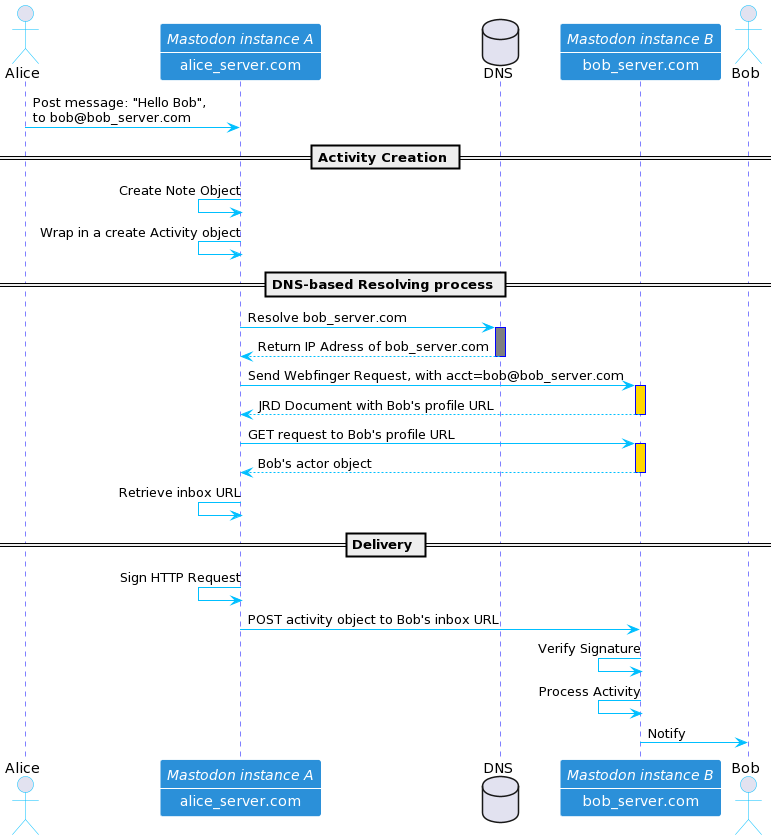
\includegraphics[width=\textwidth]{concept_and_design/normal_flow.png}
  \caption{Mastodon's implementation for the use case mentioned in \ref{section:use_case}}
  \label{fig:normal_flow}
\end{figure}

\pagebreak

% ------------Proposed Implementation------------------------------------
\section{Proposed Implementation}\label{section:did_flow}
Having seen a state-of-the-art implementation of ActivityPub for our use case, it is now imperative to address the necessary steps to make ActivityPub DID-compliant, as well as enable DIDComm as its communication protocol. 


% --------------Integrating DIDs-----------------------------
\subsection{Integrating DIDs} \label{subsec:integrating_dids}
The first question that needs to be addressed when approaching the integration of DIDs is the implications of switching from standard mastodon usernames to DIDs. Integrating DID to ActivityPub points immediately to the actor's object, as the switch would mean that the DID has to be included. Currently, most of the interactions of Mastodon via ActivityPub require the ID property to resolve to the user's profile, and therefore, to his actor's object. The simplest strategy could be, replacing the username with the DID. Thus having an ID like \verb|"www.alice_server.com/users/did:example:123456789abcdefghi"|.\\
However, there is another alternative that might work. Following the ActivityPub's specification, the ID must be a publicly dereferenceable URI, whose authority belongs to the originating server \cite{lemmer-webber_tallon_guy_prodromou_2018}. As explained in \autoref{section:dids}, a DID is a URI and it is publicly dereferenceable by nature. This allows different possibilities, to which the DID can be added. For example, using a stand-alone DID as an ID to take advantage of the discoverability of DIDs, just as proposed by Webber and Sporney in \autoref{sec:extending_activitypub}. This scenario would have the following implications. If another ActivityPub server wanted to get the user's profile URL, it would require resolving the DID to its respective DID document. This requires the DID document to include the actor's profile URL in the services section. Another option would be to add a DID URL with a query that points directly to the service endpoint that contains the actor's profile URL. Adding more precision, although still requiring a DID resolution as an intermediate step, as well as adding the service endpoint to the DID Document. Both cases are possible because ActivityPub has the \emph{URL} property that requires the actor's profile URL in case it is not in the ID property \cite{lemmer-webber_tallon_guy_prodromou_2018}. Although plausible, to prevent any unnecessary overhead a simple replacing strategy will be implemented, keeping the ID property as the profile's URL with the username replaced with the DID.

In addition to the ID, the actor's object must provide a supplementary set of URLs that point to different collections related to the user, as mentioned in \autoref{subsec:mastodon}. Following the same approach as with the ID, what if instead of using the actual URL of these collections, DID URLs pointing to the correct endpoint inside the DID Document were specified? An example for the inbox could be: \verb|"did:example:123456789abcdefghi#inbox"|.

This approach leads to the question, would it be simpler just to shift the whole actor object directly to the DID Document? This would imply that the actor object of ActivityPub is not necessary anymore and could be removed. This is also the approach Webber and Sporny proposed, mentioned in \ref{sec:extending_activitypub}. However, there are some security privacy concerns regarding the use of service endpoints in the DID Document that would advise against this. The DID specification stipulates \emph{"revealing public information through services, such as social media accounts, personal websites, and email addresses, is discouraged"} \cite{sporny_longley_sabadello_reed_steele_2021}. DID Documents are stored in a publicly available VDR, therefore any personal information revealed here is for everyone to see. The usage of URLs in service endpoints might lead to involuntary leakage of personal information or a correlation between the URL and the DID subject. In the DID document proposed by these authors, listing \ref{lst:did_and_ap}, the amount of personal information displayed, which would not be otherwise inferable, already poses a privacy issue for the DID Subject. For this reason, the actor's object will remain a part of the ActivityPub protocol in this design. This would also allow the unrestricted use of all the other attributes in the actor's object to further describe its owner, such as \emph{name}, \emph{preferredUsername}, or \emph{summary} without making this information forever public in an immutable ledger.


% ------------Decentralized resolving process------------------------------------
\subsection{Decentralized Resolving Process}
As stated in the previous section, Mastodon starts the resolving process based on the username of the user. By replacing the standard username with a DID, the current resolving flow gets disrupted, as there is no domain and thus no well-known endpoints to send requests to. Nonetheless, here is where the resolvability of the DIDs comes into play. The proposed flow takes the following steps. First, the username, which now is a DID, can be resolved to its DID Document using any kind of DID resolver. The DID Document must now contain a service with the type ActivityPub and an endpoint, where the actor's object can be retrieved. This gives us 2 possibilities. On the one hand, we could add in the well-known Webfinger endpoint, which then provides us with the profile URL from the user. On the other hand, we could skip the Webfinger request and provide the profile URL directly in the DID Document. The latter looks like the most meaningful path to take. Especially when we refer to the purpose of Webfinger, which was to enable discoverability of entities represented by URIs \cite{jones_salgueiro_jones_smarr_2013}. Webfinger's purpose shares a lot of ground with the design of DIDs, nevertheless, the DID design provides a less limited structure of resolving, as it does not rely on DNS and HTTP for its functioning. For this reason, the proposed workflow will completely remove the use of the  Webfinger protocol used in Mastodon and include the URL of the user's profile in the DID Document.
 
To make the requests to the resolver a service class \emph{DidResolverService} is needed. This class will only require one parameter, which is the DID it needs to resolve, and the response will consist of a DID document in JSON format. Furthermore, to facilitate the interaction with the properties of the DID document a class \emph{DidDocument} with the methods listed in table \ref{table:did_doc_instance_methods} is also needed.

\begin{table}[!ht]
	\centering
	\begin{tabular}{|p{5cm}|p{10cm}| }
    \hline
    \multicolumn{2}{|c|}{DID document Class} \\
    \hline
    \textbf{Function} & \textbf{Description} \\
		\hline
		\hline
      initialize(attributes) &  Stores the attributes of the DID document in accesible variables\\
    \hline
      serviceEndpoint & Returns the service endpoint URL of the first service \\
    \hline
      didcommKey & Looks for a specific key in the DID document and returns a parsed instance of it \\
    \hline
	\end{tabular}
	\caption{DID document instance methods}
  \label{table:did_doc_instance_methods}
\end{table}

With DIDs, a DID resolver, a resolver service, and a class for DID documents set up, the next task is to modify the Webfinger-based resolving process of Mastodon. Mastodon has a class called \emph{ResolveAccountService}, which triggers the Webfinger requests and processes the respective responses. It takes a username in the form of \emph{username@domain} as a parameter. If the username does not have an existing account in the local database, it makes the Webfinger request. The JRD response gets parsed to find the actor URL, and a subsequent request to the username domain gets triggered to get the actor object. Finally, it parses the actor object to create an account for this user in the local database.
The new class handling the decentralized DID-based resolving process is not very different. It will be called \emph{DID::ResolveAccountService} and will also take the username parameter in the form of \emph{did:method:example}. To resolve a DID it will first make a query to the DID resolver calling the \emph{DidResolverService}, this service instantiates a new \emph{DidDocument} class with the JSON object of the response. The profile URL of the account is then retrieved using the \emph{serviceEndpoint} method. Finally, as in the previous flow, a request is made to this URL to get the actor object for further processing, finalizing the resolving process. 


% ------------Enabling DIDComm------------------------------------
\subsection{Enabling DIDComm}\label{section:enabling_didcomm}

Having introduced DIDs to Mastodon and ActivityPub, it is now possible to enable DIDComm. Taking into account the algorithm \ref{alg:didcomm_example} shown in \autoref{section:didcomm}, it is possible to derive some requirements that DIDComm imposes:

\subsubsection*{\textbf{Access to DID-Resolver}}
This is for cases where a signature needs to be verified using an external public key published in a DID document. However, as the DID-based resolving process already requires and implements a DID resolver, this requirement can be considered fulfilled. 

\subsubsection*{\textbf{Key agreement}}
DID Documents may present more than one verification method specified in them. A specific standard verification method is required to maintain compatibility between the parties involved. This means that the sender and the recipient must use the same set of keys for encryption and/or signing purposes to have a successful message exchange through DIDComm. 
Nonetheless, addressing this requirement is unproblematic because the DID specification already provides a recommendation for this. The \emph{keyAgreement} verification relationship is intended to provide the keys, which allows an entity to confidentially share information with the DID-subject using encryption \cite{sporny_longley_sabadello_reed_steele_2021}. Even though it is possible to add an extra verification relationship called DIDComm or ActivityPub that works in conjunction with our previously defined ActivityPub service, this work will comply with the recommendation using the \emph{keyAgreement} key.

\subsubsection*{\textbf{Access to private key}}
The ActivityPub server requires access to the private key of the selected verification method. The reason is, that creating a JWS, as well as decrypting a JWE requires the private key of the user performing the action. To address this requirement, the private key of the user will be stored in the Mastodon server. The implications of this decision will be discussed in the \ref{sec:confidentiality}

\subsubsection*{\textbf{JWA Compatibility}}
The ActivityPub server must be able to support the keys and the cryptographic algorithms, which the JWA includes. This means having any library that can parse them and perform signing, signature verification,  encryption, and decryption. 
This requirement raises the complexity level in implementing DIDComm. During the development of this thesis, there were no libraries that implemented the \emph{ECDH-1PU} algorithm. For this reason, this design will implement the nested JWT alternative explained in \autoref{section:didcomm}, given that various libraries support JWS and JWE in different programming languages. In addition, to prevent any further compatibility problems on the key generation side, the common widely-supported RSA key generation algorithm will be implemented, which is also supported for JWS and JWE creation \cite{jones_2_2015}. This results in the following algorithm selection JWS tokens will use an RSA 2048 key and the \emph{RS256} hash algorithm, and the JWE tokens the \emph{RSA-OAEP}\footnote{https://www.rfc-editor.org/rfc/rfc7518\#page-14} algorithm for key management with the \emph{A128CBC-HS256}\footnote{https://www.rfc-editor.org/rfc/rfc7518\#page-22} algorithm for encryption.


\subsection{Payload Definition}\label{subsec:payload_definition}

Having addressed these requirements, it is now time to define how ActivityPub and DIDComm will work together. As part of this proposal, further changes to the ActivityPub protocol itself are not in scope. However, extending it and removing the dependency on the HTTP protocol for its communication is still intended. Therefore, encapsulation rather than modification of ActivityPub within DIDComm allows for a modular approach that keeps both protocols independent from each other. The best approach would be to follow DIDComm's schema of a nested JWT, where a plain-text message is encapsulated by a JWM, following a further encapsulation inside a JWS, and so on. The result consists of our \emph{activity} object being used as the \emph{body} of the JWM, as shown in figure \ref{fig:final_env}. 

\begin{figure}[h]
  \centering
  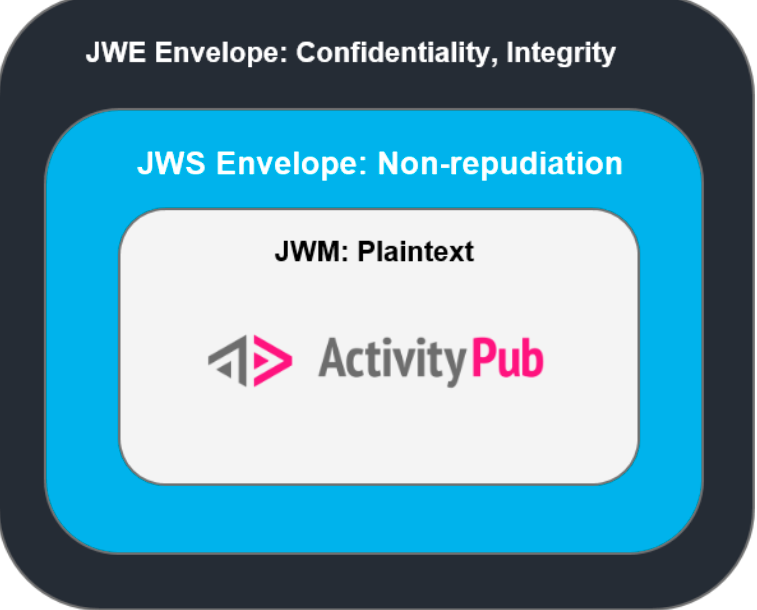
\includegraphics[width=0.4\textwidth]{concept_and_design/final_env.png}
  \caption{Proposed JWT structure using DIDComm and ActivityPub}
  \label{fig:final_env}
\end{figure}

The final nested JWT consists only of a JWE token, which is the data that will be sent. A JWE offers two types of serializations. The first one is a compact one, where all elements are concatenated in a single string separated by dots \cite{jones_hildebrand_2015}, as shown in listing \ref{lst:compact_jwe}. 

\lstset{style=JSONStyle}
\begin{lstlisting}[language=PHP, caption=JWE compact serialization \cite{jones_hildebrand_2015}, label=lst:compact_jwe, float=h!]
  BASE64URL(UTF8(JWE Protected Header)) || '.' ||
  BASE64URL(JWE Encrypted Key) || '.' ||
  BASE64URL(JWE Initialization Vector) || '.' ||
  BASE64URL(JWE Ciphertext) || '.' ||
  BASE64URL(JWE Authentication Tag)
\end{lstlisting}

The compact serialization was conceptualized in a way, that it could be used in fields with a length limit, such as HTTP headers. On the contrary, the second one offers a JSON format, which is better suited to be sent as the body of an HTTP request rather than a plain-text token. For this reason, the payload should follow the JWE JSON serialization \ref{lst:json_jwe}. Nevertheless, if the library used to create the JWE does not support the JSON format, or fails to provide access to the components of the JSON format, then the compact serialization can be implemented using the format specified in listing \ref{lst:alternative_payload}.

\lstset{style=JSONStyle}
\begin{lstlisting}[language=PHP, caption=JWE JSON serialization \cite{jones_hildebrand_2015}, label=lst:json_jwe, float=h!]
  {
    "protected":"<integrity-protected shared header contents>",
    "unprotected":<non-integrity-protected shared header contents>,
    "recipients":[
      {
        "header":<per-recipient unprotected header 1 contents>,
        "encrypted_key":"<encrypted key 1 contents>"
      },
    "aad":"<additional authenticated data contents>",
    "iv":"<initialization vector contents>",
    "ciphertext":"<ciphertext contents>",
    "tag":"<authentication tag contents>"
   }
\end{lstlisting}

\lstset{style=JSONStyle}
\begin{lstlisting}[language=PHP, caption=Alternativ payload structure, label=lst:alternative_payload, float=h!]
  { 
    "payload": "JWE with compact serialization" 
  }
   
\end{lstlisting}

To make this architecture possible, Mastodon will require the following additions. First, a class \emph{JWM}, with a setter to assign the activity object to its \emph{body}. Second, a service class called \emph{DIDCommService}, with the methods shown in table \ref{table:didcomm_service}. This service will be responsible for signing, encrypting outgoing messages, and decrypting and verifying signatures of incoming messages. 

\begin{table}[H]
  \centering
  \begin{tabular}{|p{5cm}|p{10cm}| }
    \hline
    \multicolumn{2}{|c|}{DIDComm Service Class} \\
    \hline
    \textbf{Function} & \textbf{Description} \\
    \hline
    \hline
    initialize & Takes the parameters \emph{payload, from, to,} and \emph{direction} and makes them instance variables. Parameter \emph{direction} can be \emph{incoming} or \emph{outgoing}. \\
    \hline
    getKey & It fetches a private or public key based on an account\\
    \hline
    setFromAccount & If the message is \emph{incoming}, sets the account based on the owner of the inbox URL\\
    \hline
    encrypt! & Encrypts the payload using a public key\\
    \hline
    encryptedPayload & Validates that all elements are present and then calls \emph{encrypt!} to create the JWE\\
    \hline
    decrypt! & Decrypts a JWE using a private key\\ 
    \hline
    signedPayload & Creates a JWS using a private key\\ 
    \hline
    verifiedPayloadAndSigner & Verifies the JWS using a public key. Returns the decoded payload, and the account that signed it. \\
    \hline
  \end{tabular}
  \caption{Function list for a DIDComm Service class}
  \label{table:didcomm_service}
\end{table}

Finally, a \emph{DIDCommHelper} class will be implemented in the controller area, which is the one in charge of processing incoming requests to the server. This helper will check the incoming request for the \emph{application/didcomm-encrypted+json} header. If present, it will send the payload to the \emph{DIDCommService} to set the account of the receiver, decrypt the data, verify the signature, and then forward the Activity for its standard processing. Otherwise, it will allow the unmodified payload to be processed normally.



% -------CRUD methods DID-----------------------
\subsection{CRUD Operations on a DID}\label{subsec:did_crud}

Creating a DID is rather a simple task. However, finding a DID method that allows CRUD operations to add the service endpoint and a \emph{keyAgreement} key to the DID Document, without needing to pay any GAS or any other kind of fees, is not. The following options were tested. MATTR\footnote{https://mattr.global}offers creating DIDs using \emph{did:key}, \emph{did:web} and \emph{did:ion} methods. However, they do not allow creating their keys or accessing private keys, which is necessary according to the first requirement. \emph{did:ion} offers a set of tools\footnote{https://github.com/decentralized-identity/ion-tools} to perform CRUD operations in a self-created DID and DID document. These tools are bundled in a library called ION.js, which wraps the SDK and provides an interface to interact easily with the components of ION. However, even though the \emph{update} operation is allowed, it was not possible to fetch a previously created DID and then update it, which was a necessary step. More users have encountered this issue\footnote{https://github.com/decentralized-identity/ion-tools/discussions/25}, but so far, it has not been addressed by the developers. 

An alternative to ledger-based DIDs is using the \emph{did:web} method. This method allows hosting the DID Document on any server, thus giving the server-owner full control. Nonetheless, the discovery process of this type of DID relies heavily on DNS because the DID resolver makes a GET request to the \emph{.well-known/did} endpoint of the domain in the DID to retrieve the DID document. This dependency on the domain would prevent achieving the goal of independence of centralized services.

Another DID method researched was the Uport-developed \emph{did:ethr}. Uport is now divided into two projects, namely Serto\footnote{https://serto.id} and Veramo\footnote{https://veramo.io}. Each one of them offers a decentralized identity solution. On the one hand, Serto provides a platform in the AWS Marketplace that can be easily deployed and would allow a user to create and manage DIDs from the \emph{did:ethr} method. Unfortunately, after failing to deploy the EC2 instance and contacting Serto's developers, it turned out it was temporarily not working. On the other hand, Veramo's typescript-based API allows users to manage DIDs not only in the Ethereum main network but also in other test networks such as Ropsten and Rinkeby. This allows making CRUD operations to DIDs without incurring costs. Veramo provides a setup guide\footnote{https://veramo.io/docs/node\_tutorials/node\_setup\_identifiers}, where the only thing needed externally is an Infura\footnote{https://infura.io} account to use as a Web3 Provider. Using Veramo's API will allow the creation of two different DIDs, and add the respective public keys and service endpoints.

Finally, to test this design the following elements are required. First, two DIDs for Alice and Bob respectively. Second, two servers running the Mastodon instance with the presented classes and methods implemented. One server will host the account for Alice, and the other for Bob with the respective DIDs as usernames. Third, both DID documents need to be updated with the service endpoint and the public key of the \emph{keyAgreement} keypair they were provided by the Mastodon instance. With all these elements in place, Alice can send a private message to Bob's DID, which will trigger the whole flow this design presented. Figure \ref{fig:did_flow} provides an updated diagram using the proposed DID and DIDComm-based flow. 

% Proposed Flow diagram
\begin{figure}[h]
  \centering
  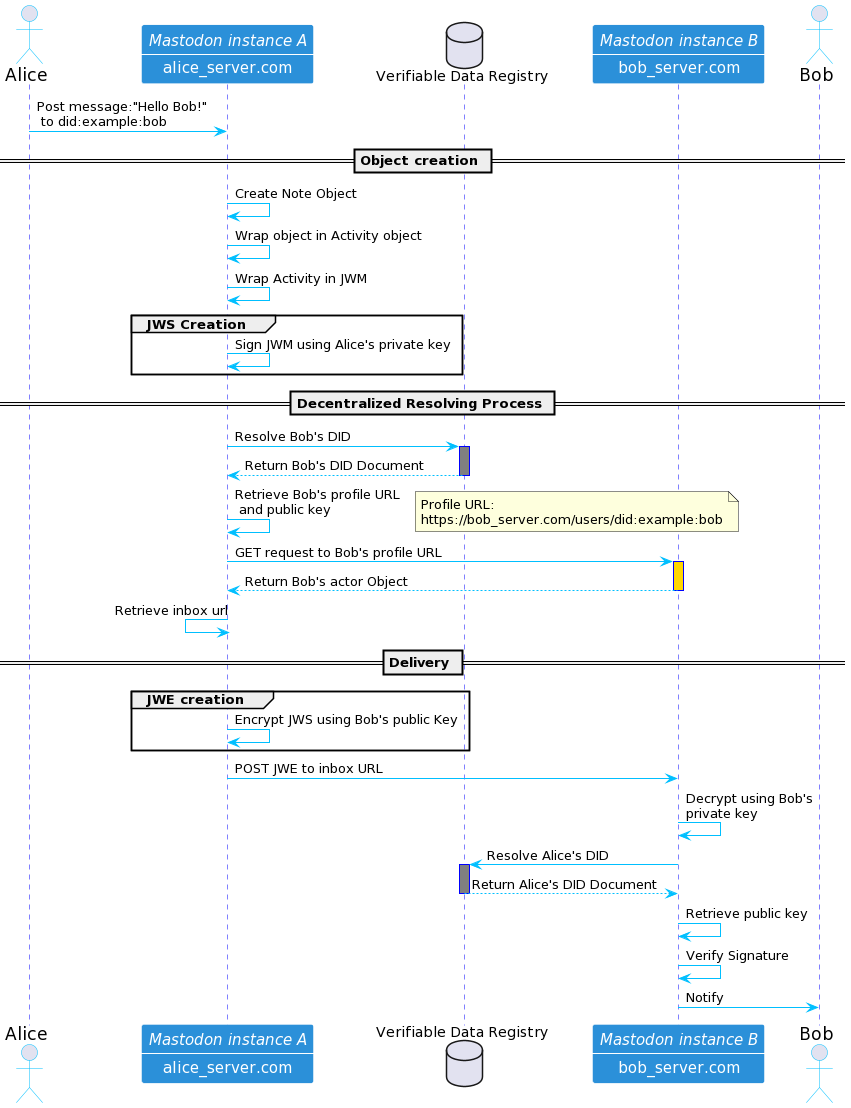
\includegraphics[height=\textheight, width=\textwidth]{concept_and_design/did_flow.png}
  \caption{DID and DIDComm flow for use case mentioned in \ref{section:use_case}}
  \label{fig:did_flow}
\end{figure}

% -------------------------------UML diagramms----------------------------------

% @startuml

% skinparam backgroundColor White

% skinparam sequence {
% ArrowColor DeepSkyBlue
% ActorBorderColor DeepSkyBlue
% LifeLineBorderColor blue
% LifeLineBackgroundColor #2b90d9

% ParticipantBorderColor White
% ParticipantBackgroundColor #2b90d9
% ParticipantFontName Impact
% ParticipantFontSize 15
% ParticipantFontColor White

% ActorFontSize 17
% ActorFontName Aapex

% }
% actor Alice as a

% participant as [
%     ====Mastodon instance A
%     ----
%     alice_server.com
% ]
% database "Verifiable Data Registry" as VDR
% participant bs [
%     ====Mastodon instance B 
%     ----
%     bob_server.com
% ]
% participant "Bob's server" as bs
% actor Bob as b

% a->as:  Post message:"Hello Bob!" \n to did:example:bob

% == Object creation ==

% as->as: Create Note Object
% as->as: Wrap object in Activity object
% as->as: Wrap Activity in JWM
% group JWS Creation
% as->as: Sign JWM using Alice's private key
% end

% == Decentralized Resolving Process ==
% as->VDR ++ #gray: Resolve Bob's DID
% VDR-->as --: Return Bob's DID Document
% as->as: Retrieve Bob's profile URL \n and public key 
% note right
% Profile URL: 
% https://bob_server.com/users/did:example:bob
% end note
% as->bs ++ #gold: GET request to Bob's profile URL
% bs-->as --: Return Bob's actor Object
% as<-as: Retrieve inbox url

% == Delivery ==
% group JWE creation
% as->as: Encrypt JWS using Bob's public Key
% end group
% as->bs: POST JWE to inbox URL

% bs->bs: Decrypt using Bob's\nprivate key
% bs->VDR ++ #gray: Resolve Alice's DID
% VDR-->bs --: Return Alice's DID Document

% bs->bs: Retrieve public key 
% bs->bs: Verify Signature

% bs->b: Notify

% @enduml

% -------Normal Flow-------------

% @startuml

% skinparam backgroundColor White

% skinparam sequence {
% ArrowColor DeepSkyBlue
% ActorBorderColor DeepSkyBlue
% LifeLineBorderColor blue
% LifeLineBackgroundColor #2b90d9

% ParticipantBorderColor White
% ParticipantBackgroundColor #2b90d9
% ParticipantFontName Impact
% ParticipantFontSize 14
% ParticipantFontColor White

% ActorFontSize 14
% ActorFontName Aapex

% }
% @startuml
% actor Alice as a
% participant as [
%     ====Mastodon instance A 
%     ----
%     alice_server.com
% ]
% database DNS
% participant bs [
%     ====Mastodon instance B 
%     ----
%     bob_server.com
% ]

% actor Bob as b

% a->as: Post message: "Hello Bob",\nto bob@bob_server.com

% == Activity Creation ==

% as<-as: Create Note Object
% as<-as: Wrap in a create Activity object

% == Resolving process ==


% as->DNS ++ #gray: Resolve bob_server.com
% DNS-->as --: Return IP Adress of bob_server.com

% as->bs ++ #gold: Send Webfinger Request, with acct=bob@bob_server.com
% bs-->as --: JRD Document with Bob's profile URL

% as->bs ++ #gold: GET request to Bob's profile URL
% bs-->as --: Bob's actor object
% as<-as: Retrieve inbox URL

% == Delivery ==
% as<-as: Sign HTTP Request
% as->bs: POST activity object to Bob's inbox URL
% bs<-bs: Verify Signature
% bs<-bs: Process Activity
% bs->b: Notify

% @enduml








% Even though there are cases when very similar domains may lead to confusion and may present some security issues. Examples of this can be found simply by comparing the most used Mastodon instance “mastodon.social” with another big\\-in\-user\-count instance such as “mstdn.social”. This type of username allows the following scenarios to play out, where differences are minimal and easily missed out, such as alice@mastodon.social and alice@mstdn.social. In addition, some users have commented that when the username is too long, the domain is not longer visible. This can be exploited by malicious actors, who may open an account in a different server with the same username as their target. Clone their profile, and try to social engineer the target's followers. 

% \lstset{style=JSONStyle}
% \begin{lstlisting}[language=PHP, caption=Alice's actor object, label=fig:alice_actor_object, float=h]

% {
% 	"@context": [
% 			"https://www.w3.org/ns/activitystreams",
% 			"https://w3id.org/security/v1",
% 	],
% 	"id": "http://alice_server.com/users/alice",
% 	"type": "Person",
% 	"following": "http://alice_server.com/users/alice/following",
% 	"followers": "http://alice_server.com/users/alice/followers",
% 	"inbox": "http://alice_server.com/users/alice/inbox",
% 	"outbox": "http://alice_server.com/users/alice/outbox",
% 	"featured": "http://alice_server.com/users/alice/collections/featured",
% 	"featuredTags": "http://alice_server.com/users/alice/collections/tags",
% 	"preferredUsername": "alice",
% 	"name": "",
% 	"summary": "",
% 	"url": "http://alice_server.com/@alice",
% 	"manuallyApprovesFollowers": false,
% 	"discoverable": false,
% 	"published": "2022-06-14T00:00:00Z",
% }


% \end{lstlisting}

% As explained in \autoref{section:didcomm}, the JWM specification defines a series of attributes that provide a starting point for the use of JWMs. Not all of these are mandatory and can thus be modified depending on the use being given to them. This gives us a lot of room to think about what is necessary and what is not. As seen in fig. (JWM with activity), redundancy can be found in each level of the JSON object. For example, the sender and recipient are defined in each layer. In the end, the Activity is the only object that will be processed, therefore, the JWM does not necessarily need any extra information, because the Activity has already all the necessary information. Furthermore, even if we wanted to use the routing mechanism of DIDComm, the attributes From and To in the JWM would only be necessary in cases where we want to send plain text messages. In addition, in almost every case the message is being sent to a specific URL, like the inbox of another user. So the receiver server will always know to whom the Activity was directed. This leaves us with a JWM structure with the attributes id and type. The requiredness of these two differs from the JWM specification and DIDComm. Nonetheless, we will stick to DIDComm and keep these two attributes compulsory. The type should be a message type URI, therefore we will use the ActivityStreams schema URI, and for the ID, we will reuse the status ID. The result is shown by figure \ref{fig:jwm_example}